%==================================================================================
%  articulo_smartcitynetV3.tex   ---  SmartCityNet, Version 3 (English, B1--B2)
%
%  "A Web Platform for Generating Optimization-Ready V2V/V2I Connectivity Data
%   from SUMO Vehicular Scenarios"
%
%  Base:  CUERPO/estructura de SmartCityNet_V3.tex + SmartCityNet_V3_Context.md;
%         PREÁMBULO tomado de articulo_smartcitynetV2 (probado, compila con MDPI).
%  Sensitivity A/B/C/D = valores REALES corridos sobre la red de Quito (output/).
%----------------------------------------------------------------------------------
%  >>> NECESITAS la carpeta  Definitions/  al lado de este .tex (clase MDPI).  <<<
%  Colores de revisión:  azul \added{} = adición V2->V3;  rojo \todo{} = pendiente.
%==================================================================================
\documentclass[engproc,proceedingpaper,submit,oneauthor]{Definitions/mdpi}

%------------------------------ MDPI internal (no modificar) -----------------------
\firstpage{1}
\makeatletter
\setcounter{page}{\@firstpage}
\makeatother
\pubvolume{1}
\issuenum{1}
\articlenumber{0}
\pubyear{2026}
\copyrightyear{2026}
\datereceived{ }
\dateaccepted{ }
\datepublished{ }

%============================== Paquetes adicionales ===============================
\usepackage[ruled,vlined,linesnumbered]{algorithm2e}
\usetikzlibrary{arrows.meta,positioning,shapes.geometric,calc,fit,backgrounds}

% ---- Colores y marcas de revisión ----
\definecolor{revisionblue}{RGB}{0,70,170}
\definecolor{todored}{RGB}{185,0,0}
\definecolor{softgray}{RGB}{246,247,249}
% \added: adiciones V2->V3 ACEPTADAS -> ya se renderizan como texto normal (negro).
\newcommand{\added}[1]{#1}
\newcommand{\todo}[1]{{\color{todored}\textbf{[TO DO: #1]}}}

% ---- Atajos matemáticos ----
\newcommand{\Atil}{\widetilde{A}}
\newcommand{\bin}[1]{\beta\!\left(#1\right)}
\newcommand{\nnz}{\operatorname{nnz}}
\newcommand{\CVR}{\mathrm{CVR}}

%============================== Portada / metadatos ================================
\Title{A Web Platform for Generating Optimization-Ready V2V/V2I Connectivity Data
from SUMO Vehicular Scenarios}

\newcommand{\orcidauthorA}{0000-0000-0000-000X}

\Author{Edison Xavier Espinel Sevilla $^{1,}$*\orcidA{}}

\AuthorNames{Edison Xavier Espinel Sevilla}

\address{%
$^{1}$ \quad Escuela Politécnica Nacional, Quito, Ecuador; edison.espinel@epn.edu.ec}

\corres{Correspondence: edison.espinel@epn.edu.ec}

% Abstract (sin líneas en blanco). En la clase MDPI \abstract es un COMANDO.
\abstract{Roadside-unit (RSU) deployment models need data that tell which vehicles
can reach each candidate RSU, in which mobility snapshot, and with how many hops.
Producing these data is not trivial: it means combining traffic mobility, urban
geometry, direct-link evaluation, graph processing, and optimization-oriented data
structures. This paper presents a web platform that turns a geographical area and a
SUMO mobility scenario into an optimization-ready connectivity dataset. The backend
integrates OpenStreetMap and SUMO tools, filters candidate RSU positions, evaluates
binary V2V and V2I links from communication range and building obstruction, and
computes cumulative and minimum-hop connectivity through a matrix recurrence.
\added{A formal proposition shows that the recurrence finds every vehicle--RSU path
within a given hop limit, and first-arrival matrices identify its minimum hop count.}
A Streamlit frontend supports configuration, execution, visualization, and export. On
the Historic Centre of Quito, varying the minimum junction degree and the clustering
radius keeps between 177 and 414 of 1211 eligible junctions as candidates (about 66\%
to 85\% reduction). The workflow separates mobility simulation from infrastructure
optimization, so the same dataset can feed different exact or heuristic deployment
models.}

\keyword{VANET; V2V connectivity; V2I connectivity; SUMO; multi-hop connectivity;
roadside units; preprocessing; facility location; operations research}

%==================================================================================
\begin{document}

%----------------------------------------------------------------------------------
\section{Introduction}

Vehicular ad hoc networks (VANETs) enable direct vehicle-to-vehicle (V2V)
communication and vehicle-to-infrastructure (V2I) communication with fixed roadside
units (RSUs), usually installed at intersections. Where these units are placed affects
coverage, path length, infrastructure cost, and network performance, so RSU deployment
is often stated as a facility-location problem and solved with exact, heuristic, or
metaheuristic methods.

These models need connectivity information \emph{before} the optimization starts:
which vehicles can reach each candidate RSU in each snapshot, and the minimum number of
relay hops. Producing it is not a minor step, as it combines traffic simulation,
vehicle-position extraction, urban geometry, range checks, obstacle detection, graph
processing, and conversion into the structures a solver accepts. Yet many deployment
studies treat these data as already available. The software side is similar: SUMO and
Python libraries are usually glued together with ad-hoc scripts, which hurts
reproducibility and reuse across formulations.

This work fills that gap with a web-based preprocessing layer that follows the
sequence
\[
\begin{aligned}
\text{urban area}\rightarrow{}&\text{SUMO snapshots}\rightarrow\text{candidate RSUs}
\rightarrow\text{V2V/V2I matrices}\\
&\rightarrow\text{minimum-hop tuples}\rightarrow\text{optimization input}.
\end{aligned}
\]
\added{Its main output is not just a set of connectivity matrices, but a traceable
dataset that keeps the relation between geographical positions, SUMO identifiers,
matrix indices, snapshots, hop counts, and optimization identifiers.} The
contributions are: (i)~a web platform that integrates a Streamlit frontend with a
Python/SUMO backend in a reproducible workflow; (ii)~automatic generation of direct
V2V and V2I matrices under a binary communication-range and line-of-sight (LoS) model;
(iii)~a configurable two-stage method that reduces the candidate RSU set using
junction degree and spatial clustering; (iv)~computation of cumulative and minimum-hop
vehicle--RSU matrices; (v)~export of optimization-ready dense structures and sparse
tuples, including an artificial no-service option per vehicle; \added{(vi)~a formal
correctness result for the recurrence and the minimum-hop representation; and (vii)~a
sensitivity analysis of how the minimum degree and clustering radius change the number
of retained candidates.} The optimization model that picks the final deployment is out
of scope: the goal is to generate its input automatically and independently of any
formulation.

%----------------------------------------------------------------------------------
\section{Related Work}\label{sec:related}

\subsection{RSU Deployment and Facility-Location Models}
RSU deployment has been studied through covering, median, routing, and stochastic
formulations. Maximal-covering models try to cover the largest demand with a limited
number of RSUs; set-covering models minimize how many units are needed to satisfy
coverage; and median-type models reduce the average distance or hop count.
Mobility-aware formulations extend these ideas over several traffic snapshots. The
stochastic model in~\citep{ref-urquiza} uses scenario-dependent connectivity tuples
and adds an artificial disconnected RSU as a no-service alternative that keeps the
problem feasible when a vehicle cannot, or should not, be assigned to a deployed real
RSU.

Despite their differences, all of these formulations rely on a common data layer:
candidate RSUs, vehicle sets, mobility scenarios, and feasible vehicle--RSU
relationships. This work focuses on producing exactly that layer. \todo{Complete
this subsection with recent studies on mobility-aware RSU placement, multi-hop
access, and exact or heuristic deployment. Every added reference must be cited in the
text.}

\subsection{SUMO-Based Platforms and Web Interfaces}
SUMO is an open-source microscopic traffic simulator with utilities to import OSM
networks, generate vehicle trips, run simulations, and export floating-car data
(FCD)~\citep{ref-sumo,ref-osm}. Streamlit and Folium support interactive Python web
interfaces and geographical visualization~\citep{ref-streamlit,ref-folium}. Their
individual capabilities are not, by themselves, the contribution of this work. The
contribution is their orchestration together with candidate filtering, geometric
direct-link evaluation, multi-hop processing, identifier traceability, and export to
optimization models.

Existing SUMO-based applications often focus on simulation control or visualization.
This platform instead treats simulation as the first stage of a data-generation
process whose final output can be consumed by facility-location and network-design
formulations. \todo{Add a short comparison with the closest scientific platforms,
considering mobility simulation, obstacle-aware V2V/V2I generation, multi-hop
processing, web interaction, optimization export, and reproducibility.}

%----------------------------------------------------------------------------------
\section{Web Platform and Connectivity-Data Generation}\label{sec:method}

\subsection{Platform Architecture and Workflow}
The platform follows a simplified model--view--controller organization. The Streamlit
frontend captures the area and the parameters, launches the workflow, and displays
maps, matrices, and summary indicators, while the Python backend prepares the SUMO
scenario, extracts snapshots, filters candidate RSUs, evaluates direct links, computes
multi-hop reachability, and exports the dataset; an orchestrator coordinates the
modules and stores each run's configuration. As shown in
Figure~\ref{fig:architecture}, OSM data become a SUMO network and building polygons
through \texttt{netconvert} and \texttt{polyconvert}, \texttt{randomTrips.py} generates
the demand, and the simulation produces the FCD snapshots that feed the connectivity
engine.

\begin{figure}[H]
\centering
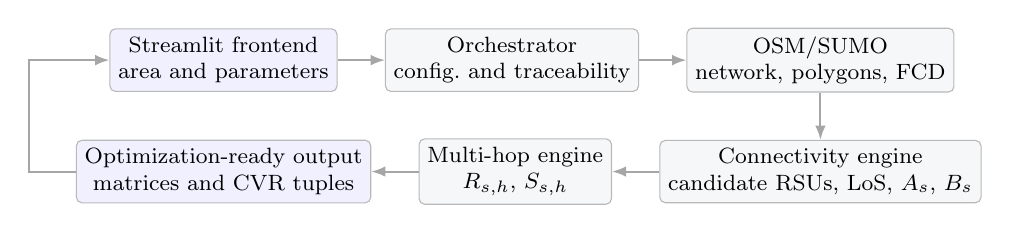
\begin{tikzpicture}[
  font=\footnotesize,
  box/.style={draw=gray!55,rounded corners=2pt,align=center,inner sep=3pt,
              minimum height=6mm,fill=softgray},
  main/.style={box,fill=blue!6},
  arr/.style={-{Latex[length=1.8mm]},gray!70,line width=.7pt}
]
\node[main] (ui) {Streamlit frontend\\area and parameters};
\node[box,right=6mm of ui] (orc) {Orchestrator\\config.\ and traceability};
\node[box,right=6mm of orc] (sumo) {OSM/SUMO\\network, polygons, FCD};
\node[box,below=6mm of sumo] (links) {Connectivity engine\\candidate RSUs, LoS, $A_s$, $B_s$};
\node[box,left=6mm of links] (hop) {Multi-hop engine\\$R_{s,h}$, $S_{s,h}$};
\node[main,left=6mm of hop] (out) {Optimization-ready output\\matrices and $\CVR$ tuples};
\draw[arr] (ui)--(orc); \draw[arr] (orc)--(sumo); \draw[arr] (sumo)--(links);
\draw[arr] (links)--(hop); \draw[arr] (hop)--(out);
% feedback: results are displayed back in the frontend (clean L on the left)
\draw[arr] (out.west) -- ++(-6mm,0) |- (ui.west);
\end{tikzpicture}
\caption{Platform architecture and end-to-end data-generation workflow.}
\label{fig:architecture}
\end{figure}

The configurable parameters are grouped into mobility settings (bounding box,
simulation duration, vehicle generation, snapshot interval, and random seed),
candidate-selection settings (minimum junction degree $g_{\min}$ and clustering radius
$\rho$), communication settings (V2V/V2I range and building obstruction), and the
maximum hop count $H$. In the case study the interface used a V2V/V2I range of
$300$~m, a $120$~s snapshot interval, $g_{\min}=4$, and $\rho=20$~m as defaults.

\subsection{Candidate RSU Selection}
SUMO can produce a large set of junctions, including intermediate road points,
internal nodes, and closely located intersections; using all of them as candidates
enlarges the search space and adds nearly equivalent positions. The platform therefore
applies a two-stage reduction: it keeps only non-internal junctions of degree at least
$g_{\min}$, then sorts them by decreasing degree and runs greedy spatial clustering,
accepting a node only when its distance to every accepted candidate exceeds $\rho$.
Because higher-degree nodes are processed first, they represent their local groups.

\begin{algorithm}[H]
\caption{Candidate RSU filtering by degree and greedy spatial clustering}
\label{alg:candidates}
\KwIn{Junction set $J$, non-internal edge set $E$, minimum degree $g_{\min}$,
clustering radius $\rho$}
\KwOut{Candidate RSU set $C$}
Initialize $\deg(j)\leftarrow 0$ for all $j\in J$\;
\ForEach{$(u,v)\in E$}{increment $\deg(u)$ and $\deg(v)$\;}
$F\leftarrow\{\,j\in J:\deg(j)\ge g_{\min}\,\}$\;
Sort $F$ by non-increasing degree; \quad $C\leftarrow\emptyset$\;
\ForEach{$j\in F$}{
  \If{$C=\emptyset$ \textbf{or} $\min_{c\in C}\operatorname{dist}(j,c)>\rho$}{
    $C\leftarrow C\cup\{j\}$\;
  }
}
\Return{$C$}\;
\end{algorithm}

This is a preprocessing heuristic, not an optimal RSU-placement algorithm. Its purpose
is to build a manageable candidate set before the deployment model is solved. Since it
may drop a location that would later be useful, the sensitivity of the retained set to
$(g_{\min},\rho)$ is reported in Section~\ref{sec:results} instead of hiding these
choices as fixed constants.

\subsection{Direct and Multi-Hop Connectivity}
For each snapshot $s\in\mathcal S$, let $\mathcal V_s=\{v_1,\ldots,v_{n_s}\}$ be the
active vehicles and $\mathcal R=\{r_1,\ldots,r_m\}$ the candidate RSUs. The binary V2V
matrix $A_s\in\{0,1\}^{n_s\times n_s}$ has $(A_s)_{ij}=1$ when $v_i$ and $v_j$ are
within the V2V range and no building polygon blocks the segment joining them; under the
bidirectional-link model it is symmetric. The binary V2I matrix
$B_s\in\{0,1\}^{n_s\times m}$ has $(B_s)_{ik}=1$ when $v_i$ can directly reach $r_k$
under the V2I range and LoS. Obstruction uses a 2-D segment--polygon intersection test,
so the result is a geometric binary approximation; it does not model attenuation,
fading, interference, or packet delivery.

A vehicle without direct V2I access may still reach an RSU through other vehicles.
Define the augmented adjacency matrix $\Atil_s=\bin{A_s+I}$, where $\beta(X)$ maps
every positive entry of $X$ to one and every zero entry to zero. Cumulative
connectivity is
\begin{align}
R_{s,1} = B_s,\qquad
R_{s,h} = \bin{\Atil_s R_{s,h-1}},\quad h=2,\ldots,H.\label{eq:rh}
\end{align}
The identity term keeps the paths already found at smaller hop counts, which gives
$R_{s,1}\le R_{s,2}\le\cdots\le R_{s,H}$ elementwise. The first-arrival matrices are
$S_{s,1}=R_{s,1}$ and $S_{s,h}=R_{s,h}-R_{s,h-1}$ for $h\ge 2$.

\begin{Proposition}\label{prop:reachability}
For any snapshot $s$, $(R_{s,h})_{ik}=1$ if and only if there is a path from vehicle
$v_i$ to candidate RSU $r_k$ using at most $h$ communication hops, where the final hop
is V2I and every previous hop is V2V.
\end{Proposition}

\begin{proof}
By induction on $h$. For $h=1$, $R_{s,1}=B_s$, so an entry is one exactly for a direct
V2I link. Assume the statement holds for $h-1$. The entry $(\Atil_s R_{s,h-1})_{ik}$
is positive if there is an index $j$ with $(\Atil_s)_{ij}=1$ and $(R_{s,h-1})_{jk}=1$.
If $j=i$, the identity term keeps a path of at most $h-1$ hops. If $j\neq i$, then
$(A_s)_{ij}=1$ adds one V2V hop from $v_i$ to $v_j$ before a path of at most $h-1$ hops
from $v_j$ to $r_k$. Conversely, every path of at most $h$ hops either already has at
most $h-1$ hops or begins with one V2V hop followed by such a path. Binarization
therefore gives exactly the stated reachability relation.
\end{proof}

\begin{Corollary}\label{cor:minhop}
For $h\ge 2$, $(S_{s,h})_{ik}=1$ if and only if the minimum number of hops from $v_i$
to $r_k$ is exactly $h$; for $h=1$, $S_{s,1}=B_s$ identifies the direct connections.
\end{Corollary}

The corollary follows from Proposition~\ref{prop:reachability} and the monotonicity of
$R_{s,h}$: each reachable vehicle--RSU pair appears for the first time at a single hop
value only. Figure~\ref{fig:matrices} shows a compact example, where the purple cells
mark the first arrival at the corresponding hop. \added{Equation~\eqref{eq:rh} uses
dense matrix multiplication followed by thresholding; a Boolean-semiring implementation
could reduce the average effort without changing the dense worst-case order, and is
left as future work.}

\begin{figure}[H]
\centering
\newcommand{\hc}[1]{\ifnum#1=1\cellcolor{violet!60}\textcolor{white}{1}\else\cellcolor{gray!8}0\fi}
\small
\begin{tabular}{c@{\hskip 6mm}c@{\hskip 6mm}c}
\begin{tabular}{c|ccc}
$R_3$ & $r_1$ & $r_2$ & $r_3$\\\hline
$v_1$ & \hc1 & \hc1 & \hc1\\
$v_2$ & \hc1 & \hc1 & \hc1\\
$v_3$ & \hc1 & \hc1 & \hc1\\
$v_4$ & \hc0 & \hc0 & \hc0
\end{tabular}&
\begin{tabular}{c|ccc}
$S_2$ & $r_1$ & $r_2$ & $r_3$\\\hline
$v_1$ & \hc0 & \hc0 & \hc1\\
$v_2$ & \hc1 & \hc1 & \hc0\\
$v_3$ & \hc0 & \hc0 & \hc1\\
$v_4$ & \hc0 & \hc0 & \hc0
\end{tabular}&
\begin{tabular}{c|ccc}
$S_3$ & $r_1$ & $r_2$ & $r_3$\\\hline
$v_1$ & \hc0 & \hc1 & \hc0\\
$v_2$ & \hc0 & \hc0 & \hc0\\
$v_3$ & \hc1 & \hc0 & \hc0\\
$v_4$ & \hc0 & \hc0 & \hc0
\end{tabular}
\end{tabular}
\caption{Illustrative cumulative ($R_3$) and first-arrival ($S_2$, $S_3$) matrices for
$H=3$. Purple cells mark the hop at which each vehicle--RSU pair first becomes
reachable; vehicle $v_4$ reaches no real RSU within the hop limit.}\label{fig:matrices}
\end{figure}

\subsection{Optimization-Oriented Export and Cardinality}
Let $K_s=\sum_{h=1}^{H}\nnz(S_{s,h})=\nnz(R_{s,H})$ be the number of reachable real
vehicle--RSU pairs in snapshot $s$. The export module creates one tuple for each real
pair at its minimum hop and one artificial no-service tuple for every active vehicle:
\[
\CVR_s=
\{\langle s,h,i,k\rangle:(S_{s,h})_{ik}=1\}
\cup
\{\langle s,H+1,i,r_\infty\rangle:i\in\mathcal V_s\}.
\]
The artificial RSU $r_\infty$ (identifier $0$) is not only physical disconnection: it
is the optimization option of leaving a vehicle unserved when real candidates are not
deployed, are saturated, or are rejected by cost or capacity constraints. It is
therefore included even when the vehicle can reach real RSUs, and is penalized at hop
$H+1$. The cardinality is $|\CVR_s|=K_s+n_s$, with $n_s\le|\CVR_s|\le n_s(m+1)$ for
$m\ge 1$; the hop limit $H$ does not multiply the real tuples, since each reachable
pair is exported once, at its minimum hop. The dataset can be written to an
OPL/\texttt{.dat} file or kept in memory for other solvers.

%----------------------------------------------------------------------------------
\section{Experimental Results}\label{sec:results}

\subsection{Experimental Settings}
The evaluation uses one real scenario in the Historic Centre of Quito, Ecuador. The
goal is not to compare cities but to measure how the candidate-generation parameters
change the size of the optimization search space while the road network stays fixed.
The two factors are the minimum junction degree $g_{\min}$ and the greedy clustering
radius $\rho$. The imported network has $1211$ eligible junctions; the SUMO run
produced $31$ snapshots (one every $120$~s) with $132$ vehicles and a $300$~m range.
All configurations reuse the same network and node-exclusion rule, which isolates the
effect of $(g_{\min},\rho)$. The study area (Figure~\ref{fig:rsumap}) corresponds to an
OpenStreetMap extract spanning about $-78.535^{\circ}$ to $-78.497^{\circ}$ longitude
and $-0.266^{\circ}$ to $-0.211^{\circ}$ latitude (UTM zone~17S, WGS84), downloaded on
5~June~2026. The pipeline ran with SUMO~1.26.0 and Python~3.14 (NumPy~2.4, pandas~3.0)
on Windows~11 (x86-64); vehicle demand was generated with \texttt{randomTrips.py} using
its default seed (no \texttt{-{}-random} flag), so the mobility is reproducible.

\subsection{Results}
Table~\ref{tab:sensitivity} reports, for four configurations, the retained candidates
$Y$ and the reduction $100(1-Y/X)$ over the $X=1211$ eligible junctions. The trend is
monotonic and matches the design of the heuristic: raising $g_{\min}$ drops low-degree
junctions before clustering, and raising $\rho$ removes candidates near an already
retained higher-degree node. The permissive setting~(A) keeps $414$ candidates
($65.8\%$ reduction), while the restrictive setting~(D) keeps only $177$ ($85.4\%$).
The reference setting~(C, $g_{\min}=4$, $\rho=20$~m) retains $333$ candidates, about a
quarter of the eligible junctions; Figure~\ref{fig:rsumap} maps these candidates over
the study area.

\begin{table}[H]
\centering
\caption{Candidate-set sensitivity in the Historic Centre of Quito
($X=1211$ eligible junctions). Values were produced by running the filtering code on
the same network.}\label{tab:sensitivity}
\begin{tabular}{ccccc}
\toprule
Config. & $g_{\min}$ & $\rho$ (m) & Candidates $Y$ & Reduction (\%)\\
\midrule
A & 3 & 15 & 414 & 65.8\\
B & 3 & 20 & 386 & 68.1\\
C & 4 & 20 & 333 & 72.5\\
D & 5 & 25 & 177 & 85.4\\
\bottomrule
\end{tabular}
\end{table}

This matters because binary deployment variables and many assignment or routing
structures grow with the number of candidate facilities. A smaller set is not
automatically better, though: it speeds up the model but may drop useful locations, so
the reduction is a preprocessing trade-off, not proof of a better deployment. On the
same scenario the platform completed the full transformation from snapshots to matrices
and tuples, producing $1390$ direct V2I contacts across the $31$ snapshots for the
$132$ vehicles and the $333$ reference candidates.

\begin{figure}[H]
\centering
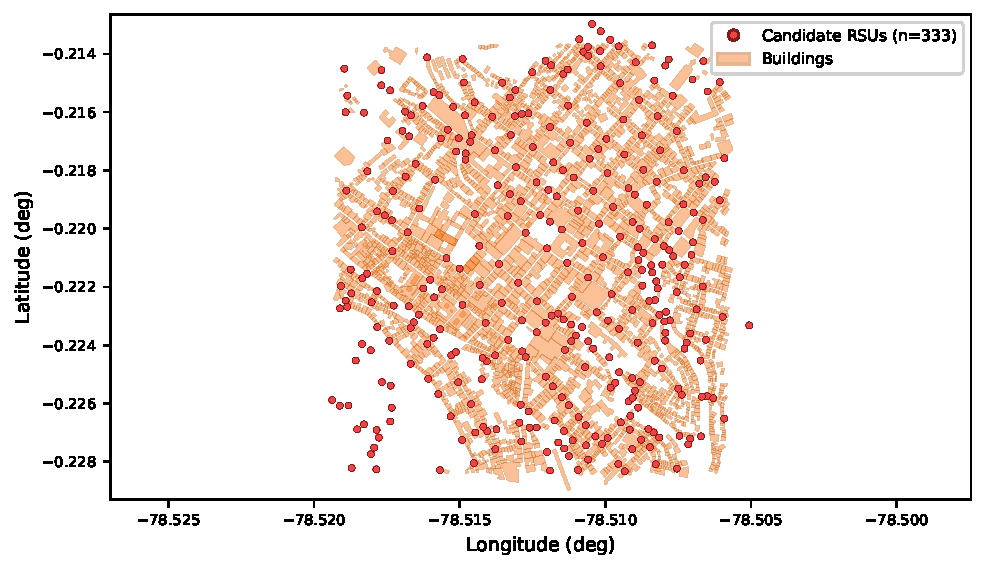
\includegraphics[width=0.6\linewidth]{fig_rsu_map.pdf}
\caption{Candidate RSUs produced by the platform for the reference configuration
(C, $g_{\min}=4$, $\rho=20$~m; $n=333$, red) over the building footprints (orange) of
the Historic Centre of Quito, in geographical coordinates.}\label{fig:rsumap}
\end{figure}

Three limitations remain: the binary geometric link model ignores path loss, fading,
interference, channel load, and packet reliability; each snapshot is processed
independently, so the recurrence describes paths \emph{inside} a snapshot, not
time-respecting store-carry-forward routes; and candidate filtering is heuristic, with
its effect on a later deployment objective still unquantified.

%----------------------------------------------------------------------------------
\section{Conclusions and Future Work}\label{sec:conclusions}

This paper presented a web platform that turns a geographical area and SUMO mobility
output into optimization-ready V2V/V2I connectivity data, combining candidate RSU
generation, direct-link evaluation with building obstruction, cumulative and
minimum-hop matrix processing, traceable identifiers, and export. A formal result
shows that the recurrence finds every vehicle--RSU relation reachable within the hop
limit, and the first-arrival matrices assign each real pair its minimum hop; the
exported set adds one artificial no-service option per vehicle, an optimization
decision rather than mere disconnection. On the Historic Centre of Quito, filtering
keeps $177$--$414$ of $1211$ eligible junctions depending on $(g_{\min},\rho)$, a
preprocessing trade-off that shrinks the model without guaranteeing a better
deployment. Future work includes comparing the recurrence against breadth-first search,
sparse and Boolean-semiring kernels, dynamic tuple generation inside the optimization
method (e.g.\ decomposition or column generation), richer propagation and reliability
models, and measuring the effect of filtering on deployment cost, coverage, capacity,
and solution time.

%----------------------------------------------------------------------------------
\authorcontributions{Conceptualization, methodology, software, validation,
writing---original draft preparation, and writing---review and editing, E.X.E.S. The
author has read and agreed to the published version of the manuscript.}

\funding{This research received no external funding.}

\dataavailability{The source code and the generated datasets (SUMO network, snapshots,
matrices, and exported tuples) are available in the project repository.}

\acknowledgments{During the preparation of this manuscript, an AI-based assistant was
used for LaTeX formatting and draft editing; the author reviewed and edited the content
and takes full responsibility for the publication.}

\conflictsofinterest{The author declares no conflict of interest.}

%----------------------------------------------------------------------------------
\reftitle{References}

\begin{thebibliography}{999}
\bibitem{ref-urquiza}
Urquiza-Aguiar, L.; Tripp-Barba, C.; Aguilar-Igartua, M. A Stochastic Optimization
Model for the Placement of Road Side Units. In {\em Proceedings of ADHOC-NOW};
Springer: Cham, Switzerland, 2016.

\bibitem{ref-sumo}
Lopez, P.A.; Behrisch, M.; Bieker-Walz, L.; et~al. Microscopic Traffic Simulation
using SUMO. In {\em Proceedings of the 21st IEEE International Conference on
Intelligent Transportation Systems}; IEEE: Maui, HI, USA, 2018; pp. 2575--2582.

\bibitem{ref-osm}
OpenStreetMap contributors. OpenStreetMap. Available online:
\url{https://www.openstreetmap.org} (accessed on 20 July 2026).

\bibitem{ref-streamlit}
Streamlit Inc. Streamlit. Available online: \url{https://streamlit.io} (accessed on
20 July 2026).

\bibitem{ref-folium}
Python Visualization. Folium: Python Data, Leaflet.js Maps. Available online:
\url{https://python-visualization.github.io/folium/} (accessed on 20 July 2026).
\end{thebibliography}

\PublishersNote{}
\end{document}
